%##################################################################################

\documentclass[12pt,a4paper,twoside]{report}
\usepackage[T1]{fontenc}
%\documentclass[12pt,a4paper,oneside]{report}
\usepackage{graphicx}
\usepackage[ngerman, english]{babel} %-- uncomment this to get english titles
%\usepackage[ngerman]{babel}
\usepackage{german,a4}
%\usepackage{picins}
%\usepackage{epsfig}
\usepackage{fancyhdr}			% for nice header and footer
\usepackage{hyperref}			% references in pdf
\usepackage[sf]{titlesec}	%customization of \chapter Titles for appendices
\usepackage{textcomp}
\usepackage{makeidx}
\usepackage{ngerman}			% german Umlauts
\usepackage[utf8]{inputenc}
\usepackage{booktabs}                               % necessary for tabulars
\usepackage[squaren]{SIunits}
\usepackage{tikz}
\usepackage[numbers,square]{natbib}
\usepackage{pgfplots}
\usetikzlibrary{shapes,arrows}
%\usepackage{wrapfig} 
%\usepackage[pdftex]{graphicx}
%\usepackage{ifthen}  
%\usepackage{booktabs} % fancy tables
%\usepackage[titletoc]{appendix} % custom naming of appendices
\usepackage{amssymb, amsmath, amsthm} % for equations & eqref
%\usepackage{listings} \lstset{basicstyle=\tiny\ttfamily, numbers=left, escapeinside={(*}{*)}, captionpos=b}
%\usepackage{dirtree}
\usepackage{acronym}
\usepackage{caption}
\usepackage{subcaption}
\usepackage{epigraph}
\usepackage{csquotes}
\usepackage{braket}
\usepackage{etoolbox}
\AtBeginEnvironment{quote}{\singlespacing\small}

%get bigger \par with one empty line
\newcommand{\mypar}{\par\medskip}

%TODO line
\newcommand{\writeTodo}{1}
\newcommand{\todo}[1]{
	\ifdefined \writeTodo
		\mypar\textbf{\textcolor{KITgreen}{TODO: }\textcolor{red}{#1}}\mypar
	\fi
} 


\newcommand{\matr}[1]{\mathbf{#1}}
%\newcommand{\matr}[1]{#1}
%\newcommand{\matr}[1]{\bm{#1}}     % ISO complying version

%\theoremstyle{plain}% default
\theoremstyle{definition}
\newtheorem{definition}{Definition}

% Abbkürzungsverzeichnis einfügen
%%%%%%%%%%%%%%%%%%%%%%%%%%%%%%%%%%%%%%%%%%%%%%%%%%%%%%%%% 
\usepackage{nomencl}
\let\abbrev\nomenclature
\renewcommand{\nomname}{Abkürzungsverzeichnis}
\setlength{\nomlabelwidth}{.25\hsize}
\renewcommand{\nomlabel}[1]{\hypertarget{nomencl-#1}{#1} }%\dotfill}
\setlength{\nomitemsep}{-\parsep}
\makenomenclature
\newcommand{\markup}[1]{\underline{\hyperlink{nomencl-#1}{#1}}}

% Farben
\usepackage{color}
\definecolor{KITgreen}{rgb}{0, .61, .51} 
\definecolor{KITbluegrey}{rgb}{.27, .39, .67} 
\definecolor{KITgrey}{rgb}{.49, .49, .49} 

% =====================================================
% Dokumenten-Platzhalter
% =====================================================
% =====================================================
% Dokumenten Platzhalter
% =====================================================


\newcommand{\titelderarbeit}{Innovative selbstlernende Gestensteuerung im Automotivbereich}
\newcommand{\artderarbeit}{Masterarbeit}

\newcommand{\diplomandprefix}{cand. el.}
\newcommand{\diplomand}{Simon Müller}

\newcommand{\betreuerA}{Marco Stang}
\newcommand{\betreuerB}{Simon Stock}

 
%\newcommand{\nameprefix}{}{}    %use no nameprefix 
\newcommand{\nameprefix}{M. Sc. }
\newcommand{\docauthor}{Simon Müller}

%\newcommand{\nameprefixb}{}{}    %use no nameprefix 
\newcommand{\nameprefixb}{M. Sc.}  
\newcommand{\docauthorb}{}

\newcommand{\nameprefixc}{}{}    %use no nameprefix 
%\newcommand{\nameprefixc}{Dipl.-Ing.}
\newcommand{\docauthorc}{}

%\newcommand{\betreuerA}{nn}
%\newcommand{\betreuerB}{nn}
\newcommand{\abgabe}{8 April 2020}
\newcommand{\versionierungsnr}{v1.0}
\newcommand{\fussnoteninhalt}{}
\newcommand{\leerzeichen}{ }

%% english version
%\newcommand{\Dachorganisation}{Karlsruhe Institute of Technology - KIT}
%\newcommand{\Institut}{Institute for Information Processing 
%												Technology - ITIV}
												
% deutsche version
\newcommand{\Dachorganisation}{Karlsruher Institut für Technologie - KIT}
\newcommand{\Institut}{Institut für Technik der Informationsverarbeitung - ITIV}

% ====================================================
% Formatierung des Dokuments
% ====================================================


%\usepackage{color}
%\usepackage{helvet}

% =====================================================
% Seite einrichten
% =====================================================
\setlength{\textwidth}{160mm} \setlength{\textheight}{235mm}
\setlength{\oddsidemargin}{5mm}
%pagelayout: (1in=25,4mm), default offset of page origin: 1in x 1in
%     25,4+5=30,4mm       160mm          19,6mm
%  |                   sadfasdfasdfasdf          |
\setlength{\evensidemargin}{-5,8mm} 
%     25,4-5,8= 19,6mm    160mm          30,4mm
%  |                   sadfasdfasdfasdf          |
\setlength{\topmargin}{0mm} \setlength{\voffset}{-15mm}
\setlength{\headsep}{12mm} \setlength{\footskip}{15mm}
\setlength{\headheight}{15.5pt}

% =====================================================
% sonstige Einstellungen
% =====================================================
%\flushbottom % Textfluss schoen unten ausrichten
\footnotesep12pt % Abstand Text / Fussnote
%\setlength{\parindent}{0pt} \setlength{\abovecaptionskip}{-6pt}
%\setlength{\belowcaptionskip}{0pt} \setlength{\intextsep}{18pt}
%\renewcommand{\baselinestretch}{1.2} % Zeilenabstand
\setcounter{secnumdepth}{4}
\newcommand{\p}[1]{\texttt{#1}}
\nonfrenchspacing

% =====================================================
% Kopf- und Fusszeile formatieren
% =====================================================
\pagestyle{fancy}
\fancyhead{}
\makeatletter
\if@twoside
	\fancyhead[LO]{\sf{\rightmark}}
	\fancyhead[RE]{\sf{\leftmark}}
	\fancyfoot[LE]{\setlength{\unitlength}{1mm}
		\begin{picture}(0,0) \put(0,-2){
			%
\includegraphics[height=0.6cm,width=0.6cm]{98_images/ITIVlogo.png}
		} \end{picture}
		%\put(9,2){\scriptsize\sf{\Institut}}\put(9,-2){\scriptsize\sf{\Dachorganisation}}}
		\put(0,2){\scriptsize\sf{\Institut}}\put(0,-2){\scriptsize\sf{\Dachorganisation}}}

\else
	\fancyhead[LO]{\sf{\leftmark}}
	\fancyfoot[LO]{\setlength{\unitlength}{1mm} 
		\begin{picture}(0,0) \put(0,-2){
			% 
\includegraphics[height=0.6cm,width=0.6cm]{98_images/ITIVlogo.png}
		} \end{picture}
		%\put(9,2){\scriptsize\sf{\Institut}}\put(9,-2){\scriptsize\sf{\Dachorganisation}}}
		\put(0,2){\scriptsize\sf{\Institut}}\put(0,-2){\scriptsize\sf{\Dachorganisation}}}
\fi
\fancyhead[LE, RO]{\sf{\thepage}}
\makeatother

\cfoot{}
\fancyfoot[RO]{\footnotesize\sf{\titelderarbeit}}
\renewcommand{\headrulewidth}{0.4pt}
\renewcommand{\footrulewidth}{1.0pt}

% ====================================================
% Kopf- und Fusszeile fuer "plain"-Format ueberschreiben
% ====================================================
\makeatletter
\if@twoside
	\fancypagestyle{plain}{%
	\fancyhf{}
	\fancyfoot[LE]{\setlength{\unitlength}{1mm}
		\begin{picture}(0,0) \put(0,-2){
			%
\includegraphics[height=0.6cm,width=0.6cm]{98_images/ITIVlogo.png}
		} \end{picture}
		%\put(9,2){\scriptsize\sf{\Institut}}\put(9,-2){\scriptsize\sf{\Dachorganisation}}}
		\put(0,2){\scriptsize\sf{\Institut}}\put(0,-2){\scriptsize\sf{\Dachorganisation}}}
	\cfoot{}
	\fancyfoot[RO]{\footnotesize\sf{\titelderarbeit}}
	\renewcommand{\headrulewidth}{0pt}
	\renewcommand{\footrulewidth}{1.0pt}}
\else
	\fancypagestyle{plain}{%
	\fancyhf{}
	\fancyfoot[L,C,R]{\setlength{\unitlength}{1mm}
	\begin{picture}(0,0) \put(0,-2){
		%
\includegraphics[height=0.6cm,width=0.6cm]{98_images/ITIVlogo.png}
	} \end{picture}
	%\put(9,2){\scriptsize\sf{\Institut}}\put(9,-2){\scriptsize\sf{\Dachorganisation}}}
	\put(0,2){\scriptsize\sf{\Institut}}\put(0,-2){\scriptsize\sf{\Dachorganisation}}}
	\cfoot{}
	\rfoot{\footnotesize\sf{\titelderarbeit}}
	\renewcommand{\headrulewidth}{0pt}
	\renewcommand{\footrulewidth}{1.0pt}}
\fi

%makes the index do not remove!
\makeindex

\hypersetup{
	%pdftex %schon gesetzt
	pdfauthor = \docauthor,
	%pagebackref,%schon gesetzt
	colorlinks=true,
	linkcolor=black,
	citecolor=black,
	urlcolor=black
	}

\providecommand{\e}[1]{\ensuremath{\times 10^{#1}}}

% =====================================================
% Inhalt der Titelseite definieren
% =====================================================

\makeindex
\newcommand{\Idx}[1]{#1 \index{#1}}

\hyphenation{
EVITA
}

% =====================================================
% Zeichen für Copyright, Trademark, Registerd, ...
% =====================================================
\def\TReg{\textsuperscript{\textregistered}}
\def\TCop{\textsuperscript{\textcopyright}}
\def\TTra{\textsuperscript{\texttrademark}}

% =====================================================
% selbs definierte Zeichen
% =====================================================
\def\zB{z.\,B. }
\def\uvm{u.\,v.\,m.}


\begin{document}

% =====================================================
% Put Titel in English
% ===================================================== 

% Inhalt der Titelseite definieren
\pagestyle{empty}
\pagenumbering{roman}
\setcounter{page}{1}

\begin{titlepage}

\begin{minipage}{15cm}
\linespread{1.2}

\begin{tabular}{lr}
\begin{minipage}{0.2\linewidth}

\includegraphics[height=1cm]{98_images/kit.png}
\end{minipage}
&
\begin{minipage}{0.8\linewidth}
\large
%\center
\vspace{7mm}
\begin{flushleft}
\Dachorganisation
\end{flushleft}
\end{minipage}
\\
\\
\begin{minipage}{0.2\linewidth}
\includegraphics[height=1cm]{98_images/ITIVLogo.png}
\end{minipage}
&
\begin{minipage}{0.8\linewidth}
\large
%\center
\vspace{7mm}
\begin{flushleft}
\Institut\\
\end{flushleft}
\end{minipage}
\\
\end{tabular}

\vspace{3cm}

\begin{center}
\Huge
\bfseries  \titelderarbeit
\end{center}

\vspace{1cm}
\begin{center}
\large 
%\subtitelderarbeit 
\vspace{1cm}
%\Large
%\textbf{\diplomandprefix\ \diplomand}

\vspace{1cm}
%\Large
%%Berichtsbezeichnung und ID Nummer
 Version 
\versionierungsnr\\
\abgabe%\textbf{\abgabe}
\end{center}
%
\vspace{2.5cm}

\begin{tabular}{rcl}
\bfseries Head of Institute:
&& Prof. Dr.-Ing. J. Becker\\
&& Prof. Dr. rer. nat  W. Stork\\
&& Prof. Dr.-Ing. Eric Sax\\
 \\
\bfseries Author:         && \diplomandprefix \leerzeichen \docauthor \\
\\
\bfseries Advisors:       &&\nameprefix  \leerzeichen \betreuerA \\
&&\nameprefixb \leerzeichen \betreuerB \\
											      \end{tabular}											
											      
\end{minipage}
\end{titlepage}
\pagestyle{fancy}
    \parindent=0pt
    %\sloppypar
    \linespread{1.2}
    \thispagestyle{plain}
    %\frontmatter
    %\maketitle

% =====================================================
% Put Titel in Deutsch
% ===================================================== 
%
% Inhalt der Titelseite definieren
\pagestyle{empty}
\pagenumbering{roman}
\setcounter{page}{1}

\begin{titlepage}

\begin{minipage}{15cm}
\linespread{1.2}

\begin{tabular}{lr}
\begin{minipage}{0.3\linewidth}

\includegraphics[height=2cm]{98_images/kit.png}
\end{minipage}
&
\begin{minipage}{0.7\linewidth}
\large
\center
Karlsruhe Institute of Technology\\
Fakultät für Elektrotechnik
\end{minipage}
\\
\\
\begin{minipage}{0.3\linewidth}
\includegraphics[height=2cm]{98_images/ITIVLogo.png}
\end{minipage}
&
\begin{minipage}{0.7\linewidth}
\large
\center
Institut für Technik der Informationsverarbeitung (ITIV)\\
\end{minipage}
\\
\end{tabular}

% #################################################################
% ### If the Title is very long reduce vspace to less than 2cm
% #################################################################
\vspace{1.5cm}

% #################################################################

\begin{center}
\Huge
\bfseries  \titelderarbeit
\end{center}

\vspace{1cm}
\begin{center}
\large 
\artderarbeit ~von\\
\vspace{1cm}
\Large
\textbf{\diplomandprefix\ \diplomand}

\vspace{1cm}
\Large
\textbf{\abgabe}
\end{center}
%
\vspace{2.5cm}

\begin{tabular}{rcl}
\bfseries Institutsleitung: 
&& Prof. Dr.-Ing. Dr. h.c. J. Becker\\
&& Prof. Dr.-Ing. Eric Sax\\
&& Prof. Dr. rer. nat  W. Stork\\

 \\
	\bfseries Betreuer:       &&\nameprefix  \betreuerA \\
											      && \betreuerB \\
\end{tabular}											
\end{minipage}
\end{titlepage}
%    \parindent=0pt
%    %\sloppypar
%    \linespread{1.2}
%    \thispagestyle{plain}
%    %\frontmatter
%    %\maketitle
%    \cleardoublepage
    
% =====================================================
% Abstract
% =====================================================     
	\begin{abstract}
		


\cleardoublepage

	\end{abstract}
	\cleardoublepage
% =====================================================
% Signaturepage
% ===================================================== 
    \chapter*{}
\begin{flushleft}
\vspace{11cm}
Erklärung\\[1cm]
Ich versichere hiermit, dass ich meine Bachelorarbeit (bzw. Masterarbeit) selbständig und unter Beachtung der Regeln zur Sicherung guter wissenschaftlicher Praxis im Karlsruher Institut für Technologie (KIT) in der aktuellen Fassung angefertigt habe. \\
Ich habe keine anderen als die angegebenen Quellen und Hilfsmittel benutzt und wörtlich oder inhaltlich übernommene Stellen als solche kenntlich gemacht.\\[1cm]

Karlsruhe, den \abgabe\\[1cm]
\end{flushleft}

\begin{center}
---------------------------------\\
\diplomand
\end{center}

	\cleardoublepage
	
	Thanks at 
\cite{Tompson2014, Yuan2017, Sun2015, Yuan2017b, GarciaHernando2017, Yuan2017c} for providing their datasets to the public.
\todo{Schöner machen!}
% =====================================================
% TOC
% ===================================================== 
    \tableofcontents
    %\clearpage
    \cleardoublepage

% =====================================================
% Main Chapters
% ===================================================== 
    %\mainmatter
    \pagenumbering{arabic}
    \setcounter{page}{1}
    \pagestyle{fancy}
 \normalsize

    
    \chapter{Introduction}

    \label{ch:Einleitung}    
    	\todo{bislang nur automatisch übersetzt}
With the increasing popularity of virtual assistants, alternative operating methods for user interfaces are increasingly being used in everyday life in the automotive sector as well. Many assistants of the current generation, however, only provide voice input.

However, especially with regard to accessibility, it is desirable to provide other input options in addition to pure voice input. However, even for people without limitations of acoustic perception, speech input is not always the optimal input method. An example of this is the multimedia control in an automobile - here voice input may already be restricted by the music being played to such an extent that traditional input methods such as control panels or touchscreens must be used. 

However, since inputs at the touch of a button or touch display can distract drivers from road traffic, additional input options that do not require the driver to turn away his eyes could additionally increase safety.

One possible solution to these problems is gesture control, in which commands are assigned to specific hand gestures. Hand gestures can be static, but can also include complex motion sequences, which are usually pre-programmed. Due to very different usage patterns, a system in which gestures can be freely defined by the user would be advantageous. 

Within the scope of this work, an innovative self-learning gesture control system for automobiles is to be developed, which makes it possible to program arbitrary hand gestures by demonstration. In a first step, the system can be pre-trained with the help of several recorded videos of different hand gestures, but the goal should be a one-shot learning, so that the user can define any gestures by showing them once.

For this purpose, a two-part system consisting of a Convolutional Neural Network (CNN) and a classifier will be used. The purpose of the CNN will be to map a depth image of the hand gesture recorded by a 3D camera (Intel Realsense) to the virtual representation of a hand, thus decisively reducing the dimensionality of the input data. The pose (or sequence of poses) is then assigned to a user-defined function using a classifier. The later goal of one-shot learning must be taken into account, which excludes algorithms that require a lot of training data. Since moving gestures may also be possible, a classifier is also required that can take this into account and assign the chronological sequence of several poses to a single gesture.

\section{Current state of research}
Research in the field of computer vision, in particular object recognition and classification, has been a strong focus in recent years \cite{FeiFei}. Especially in the field of gesture recognition there are numerous studies that investigate different strategies for segmentation and interpretation of hand and whole body gestures \cite{Zimmermann2017,Sato2001,Supancic2018,Tompson2014,Zhang2016,OhnBar2014,Ge2019,Keskin2012,Li2013,Jones2002}. 


For the segmentation two criteria usually represent a special challenge in the cited work:

Firstly, for a successful extraction of the hands from an RGB image, relevant image areas must be separated from non-relevant areas. A simple approach about the skin color as in \cite{Sato2001} is not always sufficient even when viewing in different color spaces through different skin types and light situations, which is why \cite{Zhang2016} and \cite{Li2013} additionally use a combination of different techniques such as background subtraction, viewing the texture and grouping in superpixels. Often, however, as in \cite{Sridhar2013}, an optimized background with few or no skin tones is used.

On the other hand, self occlusion during the subsequent gesture recognition is a problem that can make the recognition of certain poses more difficult. Here a fusion of depth information and RGB camera images can bring decisive advantages \cite{Keskin2012}.

The subsequent classification of poses into gestures is not dealt with further in most works, since often only pose recognition is the goal.
    \cleardoublepage
    
  	
    
    \chapter{Basics}
    \label{ch:Grundlagen}
		\section { Computer Vision }
	\subsection { Kameraparameter }
	\subsection { Segmentierung }
		

	
\section { Machine Learning }
	In den letzen Jahren gab es stetige Fortschritte in der Leistungsfähigkeit von Rechenhardware und damit einhergehend im Bereich des maschinellen Lernens (en. machine learning).
	In diesem Abschnitt werden kurz die in der Arbeit genutzten machine-learning Techniken aufgezeigt und erläutert.
	
	\subsection { Neuronale Netze }
	Künstliche Neuronale Netze (en.: artificial neural networks, kurz: ANN) sind der biologischen Funktionsweise menschlicher Nervenbahnen nachempfunden. 
	
		\subsubsection { Das Perzeptron }
		Das einlagige Perzeptron, der einfachste Fall eines neuronalen Netzes, besteht aus drei Schichten von jeweils beliebig vielen Recheneinheiten, die als Neuronen bezeichnet werden. Alle Neuronen sind dabei mit allen Neuronen der nachfolgenden Schicht über eine gewichtete Verbindung verknüpft. 
		
		Die erste Schicht übernimmt im einlagigen Perzeptron die Rolle des Eingangs. Die zweite Lage wird als "`hidden layer"' bezeichnet und die dritte Schicht stellt die berechneten Ausgangsdaten zur Verfügung.
		
		Jede Recheneinheit nimmt die Daten $o_{j-1} = o_i$ aus den vorhergehenden Neuronen entgegen und berechnet einen vorläufigen Ausgangswert $p_j$ nach Gleichung \ref{eq:perceptron_simple}. 
		
		\begin{equation}
			\label{eq:perceptron_simple}
			\text{net}_j = \sum_{i=1}^{n} w_{ij} \cdot o_i + b
		\end{equation}
		
		Die Gewichte $w_{xy}$ und Bias-Werte $b_x$ werden im Trainingsprozess anhand der Trainingsdaten optimiert und ändern sich nach dem Training nicht mehr.
		
		
		Die Summe der Produkte wird anschließend über eine nichtlineare Aktivierungsfunktion gefiltert und daraufhin in die nächste Schicht weitergereicht:
		
		\begin{equation}
		\label{eq:perceptron_act}
		o_j = \varphi\left(\text{net}_j\right)
		\end{equation}
		
		
		 
		\subsubsection { Aktivierungsfunktionen }
		Da die grundlegenden Rechenoperationen in einem neuronalen Netz linearer Natur sind, muss eine zusätzliche Nichtlinearität eingeführt werden, um auch nichtlineare Zusammenhänge erlernen zu können. 
		Hierfür werden unterschiedliche Aktivierungsfunktionen $\varphi$ eingesetzt, von denen einige häufig genutzte Funktionen im Folgenden erläutert werden.\\
		
		
		\textbf{Schwellenwertfunktion}
		Die Schwellenwertfunktion ist die ursprüngliche Aktivierungsfunktion für das Perzeptron nach \cite{McCulloch1943} und besitzt lediglich $0$ und $1$ als mögliche Ausgangswerte. Sie ist mit dem Schwellenwert $\epsilon$ definiert zu 
		\begin{equation}
		\label{eq:acti_sw}
		o_j = \left\{
		\begin{array}{ll}
		1\text{, wenn } \text{net}_j > \epsilon \\
		0 \text{ sonst}\\
		\end{array}
		\right.
		\end{equation}
		\textbf{Sigmoid}
			Die Sigmoid-Funktion ist mit einem variablen Steigungsparameter $a$ definiert zu 
			\begin{equation}
			\varphi\left(\text{net}_j\right) = \frac{1}{1+\exp(-a \cdot \text{net}_j)}
			\end{equation}
			Sie wird häufig anstatt der Schwellenwertfunktion genutzt, da sie stetig differenzierbar und somit gut geeignet für häufig genutzte Trainingsverfahren wie Gradient Descend ist.\\
			\begin{figure}[ht]
				\centering
				\begin{tikzpicture}
				\begin{axis}[
				domain=-200:200,
				xmin=-10, xmax=10,
				ymin=-1.5, ymax=1.5,
				samples=401,
				axis y line=center,
				axis x line=middle,
				]
				\addplot+[mark=none] {1/(1 + exp(-x)};
				\end{axis}
				\end{tikzpicture}
				\caption{Die Sigmoid-Funktion begrenzt die Ausgangswerte wie auch die Schwellenwertfunktion auf den Bereich [0, 1].}
				\label{fig:sigmoid_plot}
			\end{figure}


		\textbf{ReLu}
		Die Rectifying linear unit (kurz: ReLu) ist eine weitere Form der Aktivierungsfunktion, die insbesondere in Deep Neural Networks und Convolutional Neural Networks eingesetzt wird. Sie ist definiert zu
		\begin{equation}
			\label{eq:relu_def}
			\varphi(\text{net}_j) = \max(\text{net}_j, 0)
		\end{equation}
		womit negative Werte abgeschnitten werden. Im Vergleich zur Schwellenwert- bzw. Sigmoidfunktion führen große Eingangswerte hier nicht zur Sättigung (und damit kleinem Gradienten), was insbesondere in Gradientenverfahren wie in Abschnitt \ref{sec:gradient-descend} von Vorteil ist. \\
		
		\begin{figure}[ht]
			\centering
		\begin{tikzpicture}
		\begin{axis}[
		domain=-200:200,
		xmin=-10, xmax=10,
		ymin=-10, ymax=10,
		samples=401,
		axis y line=center,
		axis x line=middle,
		]
		\addplot+[mark=none] {max(x, 0)};
		\end{axis}
		\end{tikzpicture}
		\caption{Durch die ReLu-Aktivierungsfunktion werden negative Werte abgeschnitten.}
		\label{fig:relu_plot}
		\end{figure}

	
	\subsection { Spezialfälle Neuronaler Netze}
		\subsubsection { Convolutional Neural Networks (CNN) }
		Faltungsnetzwerke (en.: Convolutional neural networks, kurz CNN) sind ein Spezialfall der neuronalen Netze, der insbesondere für die Verarbeitung von höherdimensionalen Strukturen wie Bilder oder zeitliche Abfolgen von Daten geeignet ist. 
		
		In einem CNN werden zusätzlich zu den oben beschriebenen "`Dense-"' oder "`Fully-Connected-"' weitere Schichten eingesetzt, die Faltungsoperationen auf den Daten durchführen.
		
		Anstatt einer einfachen Multiplikation erfolgt in jeder Faltungsschicht eine Faltung des Eingangstensors mit einer Faltungsmatrix.
		
		Im Fall eines 2D-CNN handelt es sich bei den Eingangsdaten um eine 2D-Matrix. Eine Faltungsschicht enthält mehrere ebenfalls zweidimensionale Matrizen, die über die Eingangsmatrix geschoben werden. 
		
		
		\todo{Bild für Faltung}
		
		
		\subsubsection { Recurrent Neural Networks (RNN) }
		\subsubsection { Long Short Term Memory (LSTM) }
	
	\subsection { Trainingsmethoden }
		
		\subsubsection{Gradient Descend}
		\label{sec:gradient-descend}
		
		\subsubsection{ADAM}
		\todo{Link zum Paper ist in tensorflow source von adam optimizer zu finden}
		
	\subsection{ One Shot Learning }
	Ein Problem der bisher gezeigten Machine Learning-Methoden ist, dass sehr viele Traningsdaten benötigt werden, um die Netze ausreichend zu trainieren. In Anwendungsfällen, in denen die Trainingsdaten erst in der Benutzerinteraktion zur Verfügung stehen können jedoch häufig nicht ausreichend viele Daten gesammelt werden. Eine Möglichkeit zur Umgehung des Problems ist es, keine direkte Klassifizierung durchzuführen sondern ein Netz darauf zu trainieren, die Eingangsdaten mit einem zuvor gespeicherten Datensatz zu vergleichen. \todo{weiter}
	
\section { Anatomie der menschlichen Hand }
	Die Bewegungsfreiheit der einzelnen Handglieder unterliegt anatomischen Beschränkungen, die in der Posenschätzung nützlich sein können, um die Güte der Schätzung zu beurteilen und mit einem passenden Modell entsprechend verfeinern zu können \cite{Melax5222017}.
	
	\begin{figure}
		\centering
		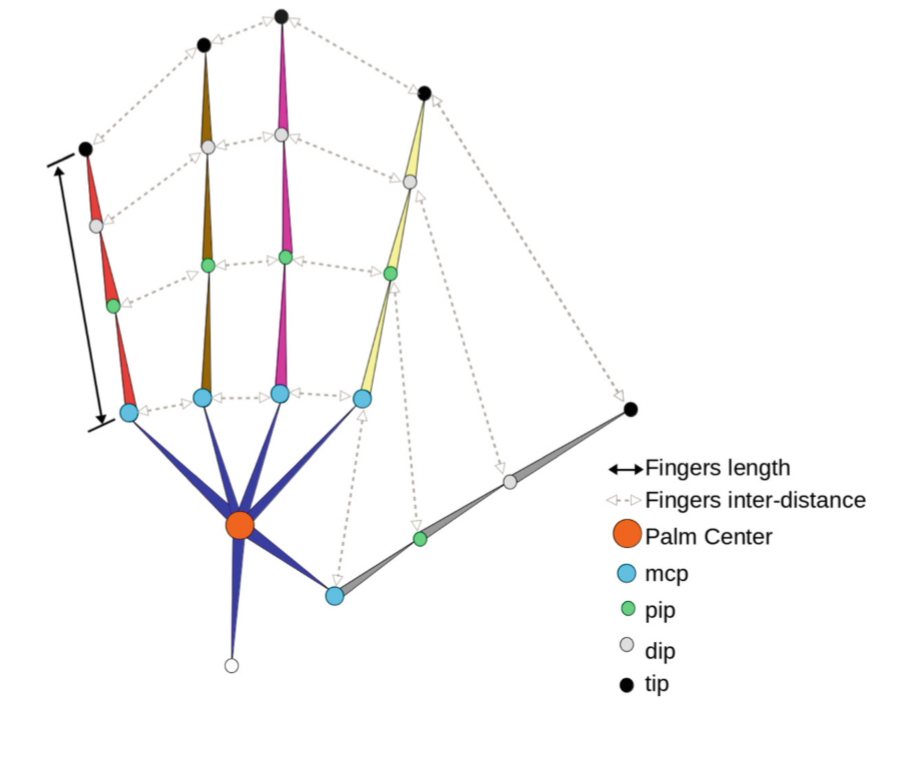
\includegraphics[width=0.7\linewidth]{Ressourcen/malik2018_hand_model}
		\caption[Handmodell nach \cite{Malik2018b}]{In \cite{Malik2018b} wird ein Modell ähnlich dem oben stehenden (Quelle: \cite{Malik2018b}) genutzt, in dem die vollständige Handpose durch 21, bzw. 22 (Gelenk-) Koordinaten bestimmt ist.}
		\label{fig:malik2018handmodel}
	\end{figure}
	
	
	\subsection{title}
	
    \cleardoublepage

	\chapter{Concept}
	\label{ch:Konzept}  	
		
\section{Hardware}
The system created in this thesis will be integrated into an existing driver cell model, which is shown im Figure \ref{fig:itiv-driver-cell} and thus has to fit certain constraints.


\subsection{Camera}

- Realsense
- Testrack


\section{Software}
In principle, it is possible to classify hand gestures directly from recorded depth information using machine learning. As in \cite{Molchanov2016}, a combination of a CNN and a downstream RNN can be used for this purpose. In this variant \todo{better formulation}, however, the structure of the network and the number and type of classes are strictly coupled. Adding, removing or changing a class would force us to retrain large parts of the network.
A further problem of this direct approach is that a sufficient amount of training data, consisting of image sequences and corresponding class labels, must be available for a reliable classification.

If new hand gestures with few example data are to be learned, and/or in the ideal case after unique Vormachen, it makes sense to divide the data processing into two sequential steps:

First, we generate a per-frame estimate of the current hand pose from the 2.5-dimensional input data (RGB-D). 


A possible time dependence of the respective hand gesture is not yet taken into account. 

\subsection{Input Format}
The camera used in this thesis, the Intel Realsense D435 provides multiple types of image streams:

\begin{itemize}
	\item An \textbf{RGB} Stream from a full HD RGB camera. 
	\item Two \textbf{infrared} image streams, provided by the two infrared modules and
	\item a \textbf{depth/disparity} map stream which is preprocessed by the camera and provides depth information with a 16 bit resolution.
\end{itemize}

For precise results it seems desirable to include all three types of input streams in the process of pose estimation in order to obtain a maximum amount of information. But in practice there are several limitations which restrict the use of the RGB and infrared streams.

Restrictions for the RGB input stream are mainly caused by the labeling process during dataset creation. Precise labeling of human hand pose datasets is impossible to achieve manually since single point of view (\markup{POV}\abbrev{POV}{Point Of View}) recordings of hand poses typically suffer from severe self-occlusion: Garcia-Hernando et al. \cite{GarciaHernando2017} count 10 occluded finger joints on average in their data set. In order to obtain reliable training data, Garcia-Hernando et al. use a body-attachable motion capturing (\markup{MoCap}\abbrev{MoCap}{Motion Capturing}) system which allows to automatically annotate the incoming image stream with precise pose information. 

While the pose information provided by this kind of automated pose annotation provides trustable pose information, it has the disadvantage that the used \markup{MoCap} system is clearly visible in the RGB images, as can be seen in Figure \ref{fig:garcia-rgb-problem}. The white cables and the tape used to fixate the sensors This bears the risk of the feature extractor overfitting on the high contrast extraneous features, rendering the trained network unusable for the intended use with bare hands. 

The infrared stream shares the same limitations but has the additional downside that to the best knowledge of the author no publicly available hand pose data set provides infrared images alongside their RGB-D data. 

The only remaining input image type is the depth map. Although the used \markup{MoCap} system might still be detectable in depth images, the contrast around the attached sensors is significantly reduced compared to the RGB images. Apart from this advantage, depth images are robust against sudden changes in illumination as long as the infrared images used to calculate the disparity are not overexposed. A third advantage that comes with disregarding RGB data is the reduced danger of overfitting on certain skin colors and thus creating a 'racist AI' \cite{Murray2019, Dietz2019, Solly2019} since depth maps provide no color information at all.

\begin{figure}
	\centering
	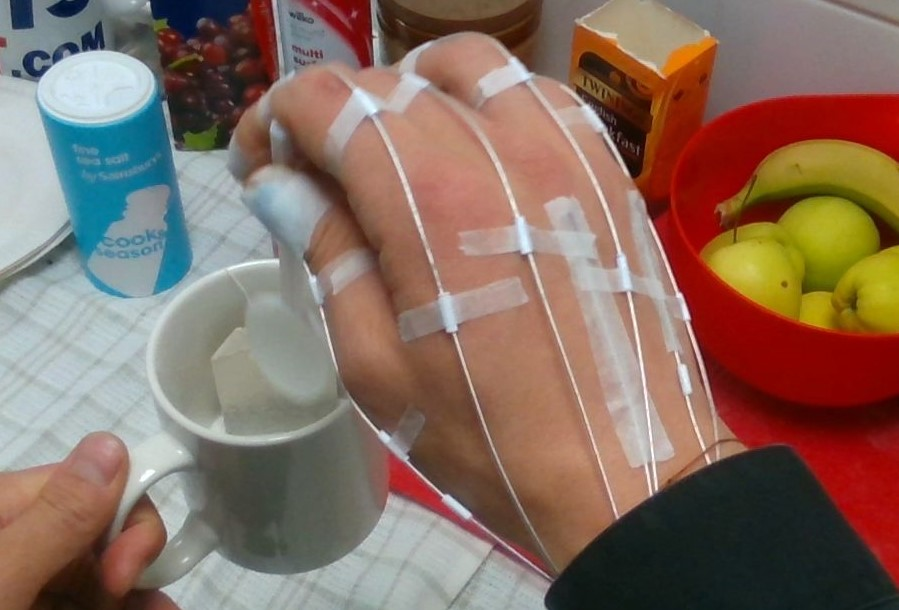
\includegraphics[width=0.7\linewidth]{Ressourcen/garcia-rgb-problem}
	\caption[Attachable motion tracking system]{Attachable motion tracking system in \cite{GarciaHernando2017}. \\ \textbf{Source:} \cite{GarciaHernando2017}}
	\label{fig:garcia-rgb-problem}
\end{figure}

\begin{figure}
	\centering
	\usetikzlibrary{arrows.meta}
\tikzset{%
	>={Latex[width=2mm,length=2mm]},
	% Specifications for style of nodes:
	base/.style = {rectangle, rounded corners, draw=black,
		minimum width=4cm, minimum height=1cm,
		text centered, font=\sffamily},
	activityStarts/.style = {base, fill=blue!30},
	startstop/.style = {base, fill=red!30},
	activityRuns/.style = {base, fill=green!30},
	process/.style = {base, minimum width=2.5cm, fill=orange!15,
		font=\ttfamily},
}
\begin{tikzpicture}[node distance=1.5cm,
    every node/.style={fill=white, font=\sffamily}, align=center]
  % Specification of nodes (position, etc.)
  \node (start)             [activityStarts]              {Activity starts};
  \node (onCreateBlock)     [process, below of=start]          {onCreate()};
  \node (onStartBlock)      [process, below of=onCreateBlock]   {onStart()};
  \node (onResumeBlock)     [process, below of=onStartBlock]   {onResume()};
  \node (activityRuns)      [activityRuns, below of=onResumeBlock]
                                                      {Activity is running};
  \node (onPauseBlock)      [process, below of=activityRuns, yshift=-1cm]
                                                                {onPause()};
  \node (onStopBlock)       [process, below of=onPauseBlock, yshift=-1cm]
                                                                 {onStop()};
  \node (onDestroyBlock)    [process, below of=onStopBlock, yshift=-1cm] 
                                                              {onDestroy()};
  \node (onRestartBlock)    [process, right of=onStartBlock, xshift=4cm]
                                                              {onRestart()};
  \node (ActivityEnds)      [startstop, left of=activityRuns, xshift=-4cm]
                                                        {Process is killed};
  \node (ActivityDestroyed) [startstop, below of=onDestroyBlock]
                                                    {Activity is shut down};     
  % Specification of lines between nodes specified above
  % with aditional nodes for description 
  \draw[->]             (start) -- (onCreateBlock);
  \draw[->]     (onCreateBlock) -- (onStartBlock);
  \draw[->]      (onStartBlock) -- (onResumeBlock);
  \draw[->]     (onResumeBlock) -- (activityRuns);
  \draw[->]      (activityRuns) -- node[text width=4cm]
                                   {Another activity comes in
                                    front of the activity} (onPauseBlock);
  \draw[->]      (onPauseBlock) -- node {The activity is no longer visible}
                                   (onStopBlock);
  \draw[->]       (onStopBlock) -- node {The activity is shut down by
                                   user or system} (onDestroyBlock);
  \draw[->]    (onRestartBlock) -- (onStartBlock);
  \draw[->]       (onStopBlock) -| node[yshift=1.25cm, text width=3cm]
                                   {The activity comes to the foreground}
                                   (onRestartBlock);
  \draw[->]    (onDestroyBlock) -- (ActivityDestroyed);
  \draw[->]      (onPauseBlock) -| node(priorityXMemory)
                                   {higher priority $\rightarrow$ more memory}
                                   (ActivityEnds);
  \draw           (onStopBlock) -| (priorityXMemory);
  \draw[->]     (ActivityEnds)  |- node [yshift=-2cm, text width=3.1cm]
                                    {User navigates back to the activity}
                                    (onCreateBlock);
  \draw[->] (onPauseBlock.east) -- ++(2.6,0) -- ++(0,2) -- ++(0,2) --                
     node[xshift=1.2cm,yshift=-1.5cm, text width=2.5cm]
     {The activity comes to the foreground}(onResumeBlock.east);
  \end{tikzpicture}
	\caption{}
	\label{fig:software-net-structure-blackbox}
\end{figure}

\subsection{Training}
	Aufgrund des zweistufigen Aufbaus kann auch das Training des Netzes in zwei Stufen erfolgen.



\section{Datasets and Data Generation}
Training the pose estimation module requires a large amount of sample data to cover as many hand poses as possible. A valid data set for the given task consists of the following data:
\begin{itemize}
 \item A depth map, containing the subject's right hand in any pose. 
 \item A set of at least 21 hand joint annotations, describing the 3d position of each joint. The resulting hand model is depicted in Figure \ref{fig:malik2018handmodel}.
\end{itemize}

The data sets published in \cite{Tompson2014, Yuan2017, Sun2015, Yuan2017b, GarciaHernando2017, Yuan2017c} provide the needed information together with additional labels for sequences of hand poses, describing the gesture/action depicted in each sequence. Since the aforementioned data sets provide their data in different formats, they have to be unified before they can be used for the training process. 

Tensorflow provides the possibility to store training data in a serialized representation which increases load times for each data pair significantly. 

\todo{Data load time comparison: tfrecord, tf with single files, python with single files}

    \cleardoublepage    
    
    \chapter{Implementation}
    \label{ch:implementierung}   
   		\section{Hand pose estimation}
For the task of estimating the user's hand pose, we implement two different hand pose regressors and compare their performance. 

For both regressors, we use ImageNetV2 \cite{Sandler} as an encoder to transfer the given depth data into a latent feature space. 

\subsection{Structural training}
As described in the previous section, the hand pose module uses an encoder to convert the high-dimensional input data into a latent feature space. 
Using the principle of transfer learning, we can train the encoder separately in order to improve the overall performance of the pose regression network. 

For this we use an auto encoder-like structure as shown in Figure \ref{fig:autoencoder}.


\section{Gesture Classification}
\section{Physical Construction}

   		
    \chapter{Evaluation}
	\label{ch:Bewertung}  
		\input{05_diskussion/diskussion.tex}
    \cleardoublepage    

    \chapter{Fazit}
    \label{ch:Fazit}    
    	\input{06_fazit/fazit.tex}
    \cleardoublepage
    
% =====================================================
% Bibliography
% ===================================================== 
%\nocite{*}

%====== DATASETS
\nocite{Tompson2014, Yuan2017, Sun2015, Yuan2017b, GarciaHernando2017, Yuan2017c}

%\addcontentsline{toc}{chapter}{Literaturverzeichnis, in ToC löschen}
%\addcontentsline{toc}{chapter}{Literature}
%\bibliographystyle{dinat}        % use a DIN style for the bibliography
%\bibliographystyle{plain}        % use a DIN style for the bibliography
%\bibliographystyle{abbrv}			%mit nummern in []
%\bibliographystyle{plain}			%mit nummern in []
%\bibliographystyle{alpha}			%3 Buchstaben + Jahr
%\bibliographystyle{alphadin}
\bibliographystyle{IEEEtran}

    % use external Bib-File, 
		\bibliography{99_bib/standardbib}
		\cleardoublepage
% =====================================================
% Appendix
% ===================================================== 
    \appendix

%    \input{95_anhang/anhang}
		\cleardoublepage

    \listoftables
    	\cleardoublepage
    \listoffigures
    	\cleardoublepage
    \printindex
    	\cleardoublepage
    \printnomenclature
    \renewcommand{\leftmark}{\uppercase{Abkürzungsverzeichnis}}
    	\cleardoublepage

\end{document}

